\documentclass{standalone}

\usepackage{tikz}
\usetikzlibrary{shapes, snakes, patterns, arrows}
\usetikzlibrary{calc}
\usepackage{pgfplots}
\usepgfplotslibrary{fillbetween}
\usepackage{amsmath}
\usepackage{amssymb}
\usepackage{amsfonts}

\begin{document}
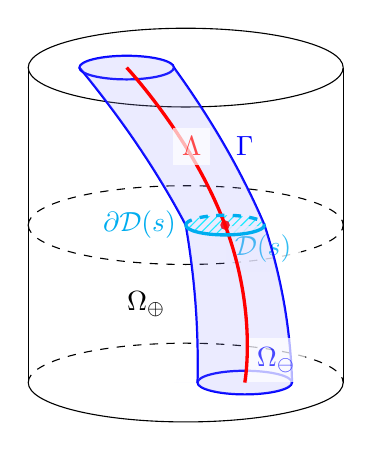
\begin{tikzpicture}


% Omega
\draw[] (0, 2) ellipse (2. and 0.5);
\draw (-2.,2) -- (-2.,-2);
\draw (-2.,-2) arc (180:360:2. and 0.5);
\draw [dashed] (-2.,-2) arc (180:360:2. and -0.5);
\draw (2.,-2) -- (2., 2);
% Top whole
\draw[blue, thick] (-0.75, 2) ellipse (0.6 and 0.15);
% Bottom whole
\draw[blue, thick] (0.75, -2) ellipse (0.6 and 0.15);
% Auxliary middle surface
\draw [dashed, thin](-2., 0) arc (180:360:2. and 0.5);
\draw [dashed, thin] (-2.,0) arc (180:360:2. and -0.5);

\fill[pattern color=cyan, pattern=north east lines] (0.5, 0) ellipse (0.5 and 0.125);
\node [cyan, below right, fill=white, opacity=0.8] at (0.5, 0.0) {$\mathcal{D}(s)$};

\node[mark size=1.5pt, color=red] at (0.5, 0.0) {\pgfuseplotmark{*}};


% Walls of gamma
\draw [blue, thick, name path global = topleft] plot [smooth, tension=1] coordinates { (-1.35,2) (-0.6, 1) (0,0)};
\draw [blue, thick, name path global = botleft] plot [smooth, tension=1] coordinates { (0,0) (0.125, -1) (0.15,-2)};

\draw [blue, thick, name path global = topright] plot [smooth, tension=1] coordinates { (-0.15,2) (0.5, 1) (1.0,0)};
\draw [blue, thick, name path global = botright] plot [smooth, tension=1] coordinates { (1.0,0) (1.25, -1) (1.35,-2)};

%\fill [gray, opacity=0.5] (-1.25,0) -- (-1.25,-3.5) arc (180:360:1.25 and 0.5) -- (1.25,0) arc (0:180:1.25 and -0.5);

\tikzfillbetween[of=topleft and topright]{blue!40!white, opacity=0.2};
\tikzfillbetween[of=botleft and botright]{blue!40!white, opacity=0.2};
\fill[blue!40!white, opacity=0.2] (-1.35, 2) arc (180:360:0.6 and -0.15) -- (-0.75, 2);
\fill[blue!40!white, opacity=0.2] (0.15, -2) arc (180:360:0.6 and 0.15) -- (-0.15, -2);
\node[blue, fill=white, opacity=0.7, above] at (1.15, -2) {$\Omega_{\ominus}$};

% Curve
\draw [very thick, red] plot [smooth, tension=1] coordinates { (-0.75,2) (0.5, 0) (0.75,-2)};
\node[red, fill=white, opacity=0.7] at (0.075, 1) {$\Lambda$};

\node[] at (-0.5, -1) {$\Omega_{\oplus}$};

\node[blue] at (0.75, 1) {$\Gamma$};

%\fill [white!50!blue, opacity=0.5] (-1.,0) -- (-1.,-3.5) arc (180:360:1. and 0.3) -- (1., 1) arc (0:180:1. and -0.3);
%% % Outer guy
%% \draw (0,0) ellipse (1.25 and 0.5);
%% \draw (-1.25,0) -- (-1.25,-3.5);
%% \draw (-1.25,-3.5) arc (180:360:1.25 and 0.5);
%% \draw [dashed] (-1.25,-3.5) arc (180:360:1.25 and -0.5);
%% \draw (1.25,-3.5) -- (1.25,0);  
%% \fill [gray, opacity=0.5] (-1.25,0) -- (-1.25,-3.5) arc (180:360:1.25 and 0.5) -- (1.25,0) arc (0:180:1.25 and -0.5);
%% %
%% \draw [red, thick] (0, -3.5, 0) -- (0, 1.7);
%% \node [right, blue] at (0, 1.7) {$\vec{n}$};
%% \node [right] at (0, -1.5) {$\Lambda$};
%% %
%% \node [below, gray] at (0, -4) {$\Omega$};
%% %
%% \node [right, blue] at (0, 1) {$y$};
%% \draw [very thick, blue, ->] (0, 1) -- (0, 1.5);

%% \node [right, blue] at (1, 1) {$\mathcal{C}_R(y)$};
%% \draw [dashed] (0, 1) -- (-1, 1);
%% \node [above] at (-1, 1.1) {$R$};
%% \node[mark size=1.5pt, color=blue] at (0, 1) {\pgfuseplotmark{*}};
% Middle whole
\draw [very thick, cyan] (0, 0) arc (180:360:0.5 and 0.125);
\draw [very thick, dashed, cyan] (0,0) arc (180:360:0.5 and -0.125);
\node [left, cyan] at (0, 0) {$\partial\mathcal{D}(s)$};

%\node[left] at (0, -2) {$\partial\Omega$};
%\node[right] at (0, 2) {$\partial\Omega$};
%\node[right] at (2, 1) {$\partial\Omega$};

\end{tikzpicture}
\end{document}
